%% wheelchart.tex
%% Copyright 2022 Matthias Floré
%
% This work may be distributed and/or modified under the
% conditions of the LaTeX Project Public License, either version 1.3c
% of this license or (at your option) any later version.
% The latest version of this license is in
%   http://www.latex-project.org/lppl.txt
% and version 1.3c or later is part of all distributions of LaTeX
% version 2005/12/01 or later.
%
% This work has the LPPL maintenance status `maintained'.
% 
% The Current Maintainer of this work is Matthias Floré.
%
% This work consists of the files wheelchart.pdf, wheelchart.sty,
% wheelchart.tex and README.md.
\documentclass[a4paper,english,dvipsnames]{ltxdoc}
\usepackage[english]{babel}
\usepackage{graphicx}
\usepackage[a4paper,left=2.25cm,right=2.25cm,top=2.5cm,bottom=2.5cm,nohead]{geometry}
\usepackage{parskip}
\usepackage[T1]{fontenc}
\usepackage[utf8]{inputenc}
\usepackage{mathtools}
\usepackage{amssymb}
\usepackage{interval}
\allowdisplaybreaks
\usepackage{siunitx}
\usepackage{etoolbox}
\usepackage{listofitems}
\usepackage{wheelchart}
\usetikzlibrary{decorations.markings,patterns}
\input{pgfmanual-en-macros.tex}
\usepackage[page]{totalcount}
\usepackage{fancyhdr}
\pagestyle{fancy}
\renewcommand{\headrulewidth}{0pt}
\cfoot{\iftotalpages\begin{tikzpicture}[scale=0.15]\wheelchart[data={},gap,middle=\thepage,slices style={/utils/exec={\ifnum\thepage=\WCcount\def\WCcolor{Cyan}\else\def\WCcolor{Gray}\fi},\WCcolor},total count={\totalpages-1},value=1]{}\end{tikzpicture}\fi}
\fancyhead{}
\usepackage{etoc}
\def\WCtableofcontents{}
\etocsetstyle{section}{}{}{\xappto\WCtableofcontents{,\etocthename/\etocthenumber/\etocthepage}}{}
\etocsettocstyle{\hypersetup{hidelinks}}{}
\etocglobaldefs
\usepackage{imakeidx}
\makeindex[program=makeindex,columns=2,intoc=true]
\indexsetup{othercode={\thispagestyle{fancy}}}
%\PassOptionsToPackage{hyphens}{url}
\usepackage{xurl}
\usepackage[linktoc=all,pdfstartview=FitH,colorlinks=true,linkcolor=Mahogany,citecolor=ForestGreen,urlcolor=MidnightBlue,bookmarksnumbered=true]{hyperref}
\hypersetup{pdftitle={The wheelchart package},pdfauthor={Matthias Flor\'e},pdfsubject={Manual},pdfkeywords={wheelchart}}
\setcounter{tocdepth}{2}
\setcounter{secnumdepth}{2}
\title{The \texttt{wheelchart} package\\[12pt]\large Draw wheelcharts with \tikzname}
\author{Matthias Flor\'e}
\date{Version 1.0 (2022/09/11)}%\\[12pt]
\begin{document}
\maketitle
\thispagestyle{fancy}
\begin{abstract}
\noindent This package is based on the package |tikz| (see \cite{TtTaPGFp}) and can be used to draw wheelcharts with \tikzname. It provides several options to customize the wheelcharts. Other tools for creating wheelcharts or pie charts can be found in \cite{MpMP}, \cite{JhcIparowcltopotPGFm}, \cite{Tumfdb}, \cite{RSVpaaMfp} and \cite{XdPCbupp}.% This is the manual for version .
\end{abstract}
\section*{\contentsname}
\tableofcontents
\patchcmd{\WCtableofcontents}{,}{}{}{}
\begin{codeexample}[]
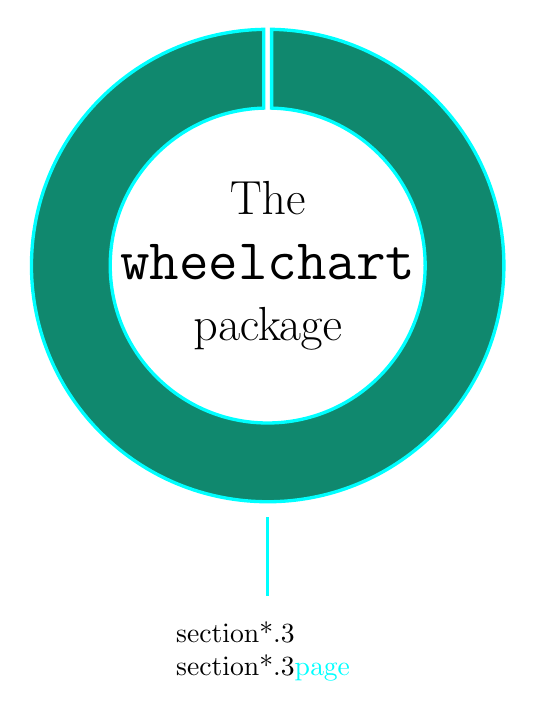
\begin{tikzpicture}
\wheelchart[
    data={%
\pgfmathsetmacro{\WCcolornumber}{(\WCcount/\WCtotalcount)*100}%
\ifdefempty{\WCvarB}{\gdef\WChyperlink{section*.3}}{\gdef\WChyperlink{section.\WCcount}}%
\hyperlink{\WChyperlink}{%
\textbf{\textcolor{PineGreen!\WCcolornumber}{\Large\ifdefempty{\WCvarB}{}{\WCvarB{} }\WCvarA}}}\\%
\hyperlink{\WChyperlink}{\textcolor{Cyan}{page \WCvarC}}%
},
    gap,
    lines,
    lines style={Cyan,very thick},
    middle={\LARGE The\\[10pt]\huge\texttt{wheelchart}\\[10pt]\LARGE package},
    slices style={
        /utils/exec={\pgfmathsetmacro{\WCcolornumber}{(\WCcount/\WCtotalcount)*100}},
        PineGreen!\WCcolornumber,
        draw=Cyan,
        very thick
    },
    value=1
]{\WCtableofcontents}
\end{tikzpicture}
\end{codeexample}
\section{Usage}
The package |wheelchart| can be used by putting the following in the preamble.
\begin{codeexample}[code only]
\usepackage{wheelchart}
\end{codeexample}
The package |wheelchart| loads the package |tikz| and the \tikzname{} library |calc|.

Many examples in this manual use colors which can be defined by giving |dvipsnames| as an option to |\documentclass|.
\section{The main macro}
\begin{command}{\wheelchart\opt{\oarg{options}}\marg{wheelchart data}}
This command can be placed inside a |tikzpicture| environment. It draws a wheelchart with \meta{wheelchart data}. The \meta{wheelchart data} is a comma separated list. Each item in this list corresponds to one slice of the wheelchart and consists of data separated by a |/|. The precise syntax of the \meta{wheelchart data} will be explained below. The \meta{options} can be given with the keys described in Section \ref{Keys}.
\begin{command}{\exampleforthismanual}
To simplify the creation of examples in this manual, we define the \meta{wheelchart data} below.
\begin{codeexample}[]
\gdef\exampleforthismanual{%
14/Apricot/Apricot/{A, B, C, E, K}/{north east lines}/0/0/Gray,
40/LimeGreen/Lime/{B, C}/grid/0/15/Black,
20/Melon/Melon/{A, C}//0.5/0/none,
16/OliveGreen/Olive/{A, B, E, K}/dots/0/0/none,
28/Peach/Peach/{A, B, C, E, K}/{fivepointed stars}/0/0/Lavender,
32/Plum/Plum/{A, B, C, E, K}/bricks/0/{-15}/none,
50/WildStrawberry/Strawberry/{B, C, E, K}//1/0/DarkOrchid%
}
\end{codeexample}%pattern crosshatch,checkerboard
\end{command}
The default wheelchart with these data is shown below.
\begin{codeexample}[width=10cm]
\begin{tikzpicture}
\wheelchart{\exampleforthismanual}
\end{tikzpicture}
\end{codeexample}
\end{command}
\section{Additional macros}
\begin{command}{\WCcount}
This macro gives the current number of the slice in the \meta{wheelchart data}.
\begin{codeexample}[width=10cm]
\begin{tikzpicture}
\wheelchart[
    inner data=\WCcount
]{\exampleforthismanual}
\end{tikzpicture}
\end{codeexample}
\end{command}
\begin{command}{\WCdataangle}
This macro stores the sum of the value of the key |data angle shift| (taking into account the key |counterclockwise|) and the macro |\WCmidangle| modulo $360$.
\end{command}
\begin{command}{\WCmidangle}
This macro gives the angle in degrees modulo $360$ of the middle of the current slice.
\begin{codeexample}[width=10cm]
\begin{tikzpicture}
\wheelchart[
    data angle shift=\WCvarG,
    data style={
        rotate=\WCdataangle,
        draw=Magenta,
        fill=GreenYellow,
        anchor=west,
        text=Gray
    }
]{\exampleforthismanual}
\wheelchart[
    data={},
    inner data={%
        \textbackslash WCmidangle%
    },
    inner data style={
        rotate=\WCmidangle,
        font=\ttfamily
    },
    slices style={fill=none}
]{\exampleforthismanual}
\end{tikzpicture}
\end{codeexample}
\end{command}
\begin{command}{\WCperc}
This macro displays |\WCpercentage| rounded up to the number of decimals determined by the key |perc precision| followed by a \unit{\percent} symbol.

If the package |siunitx| is loaded then the following code is used. The package |siunitx| can be loaded before or after the package |wheelchart|.
\begin{codeexample}[code only]
\qty[round-mode=places,
     round-precision=\pgfkeysvalueof{/wheelchart/perc precision}]{\WCpercentage}{\percent}
\end{codeexample}
If the package |siunitx| is not loaded then the following code is used.
\begin{codeexample}[code only]
\WCpercentagerounded\,\%
\end{codeexample}
\end{command}
\begin{command}{\WCpercentage}
This macro gives the percentage of the current slice where the total is computed with the values of the key |value|. Note that rounding errors can occur.
\begin{codeexample}[]
\begin{tikzpicture}
\wheelchart[
    data={\WCvarC\\\WCperc},
    slices style={
        /utils/exec=\pgfmathsetmacro{\WCcolornumber}{4*\WCpercentage},
        \WCvarB!\WCcolornumber
    }
]{\exampleforthismanual}
\end{tikzpicture}
\end{codeexample}
\end{command}
\begin{command}{\WCpercentagerounded}
This macro displays |\WCpercentage| rounded up to the number of decimals determined by the key |perc precision|.
\end{command}
\begin{command}{\WCtotalcount}
This macro gives the total number of slices.
\end{command}
\begin{command}{\WCtotalnum}
This macro gives the sum of all values of the key |value|.
\begin{codeexample}[width=10cm]
\begin{tikzpicture}
\wheelchart[
    data={\WCvarC: \WCvarA},
    middle={%
        \textbf{\huge Fruit}\\%
        \WCtotalcount{} species\\%
        \pgfmathprintnumber{\WCtotalnum}
        pieces%
    }
]{\exampleforthismanual}
\end{tikzpicture}
\end{codeexample}
\end{command}
\begin{command}{\WCvarA}
\end{command}
\begin{command}{\WCvarB}
\end{command}
\begin{command}{\WCvarC}
\end{command}
\begin{command}{\WCvarD}
\end{command}
\begin{command}{\WCvarE}
\end{command}
\begin{command}{\WCvarF}
\end{command}
\begin{command}{\WCvarG}
\end{command}
\begin{command}{\WCvarH}
\end{command}
\begin{command}{\WCvarI}
\end{command}
\begin{command}{\WCvarJ}
\end{command}
\begin{command}{\WCvarK}
\end{command}
\begin{command}{\WCvarL}
\end{command}
\begin{command}{\WCvarM}
\end{command}
\begin{command}{\WCvarN}
\end{command}
\begin{command}{\WCvarO}
\end{command}
\begin{command}{\WCvarP}
\end{command}
\begin{command}{\WCvarQ}
\end{command}
\begin{command}{\WCvarR}
\end{command}
\begin{command}{\WCvarS}
\end{command}
\begin{command}{\WCvarT}
\end{command}
\begin{command}{\WCvarU}
\end{command}
\begin{command}{\WCvarV}
\end{command}
\begin{command}{\WCvarW}
\end{command}
\begin{command}{\WCvarX}
\end{command}
\begin{command}{\WCvarY}
\end{command}
\begin{command}{\WCvarZ}
The \meta{wheelchart data} in the command |\wheelchart| is a comma separated list. Each item in this list corresponds to one slice of the wheelchart and consists of data separated by a |/|. These individual data are interpreted as |\WCvarA/\WCvarB/\WCvarC/...| and can be accessed within the \meta{options} of the command |\wheelchart| by the macros |\WCvarA| till |\WCvarZ| except within the keys |at|, |caption|, |caption left|, |caption left style|, |caption style|, |contour|, |counterclockwise|, |expand list|, |middle fill|, |name|, |start angle|, |start half|, |title|, |title left|, |title left style|, |title style|, |total angle| and |total count|. Thus up to 26 data can be given to each slice of the wheelchart.

Initially, only |\WCvarA|, |\WCvarB| and |\WCvarC| are used for |value=\WCvarA|, |slices style=\WCvarB| and |data=\WCvarC|.
\begin{codeexample}[width=10cm,preamble={\usetikzlibrary{patterns}}]
\begin{tikzpicture}
\wheelchart[
    data={},
    gap,
    radius={0.5}{3},
    slices style={\WCvarB!70,draw=\WCvarH,ultra thick,pattern=\WCvarE,pattern color=\WCvarB!70},
    value=1,
    wheel data=\WCvarC,
    %wheel data style={shift={(\WCmidangle:0.5)}},
    %wheel data pos=0.5
]{\exampleforthismanual}
\wheelchart[
    data={\textcolor{\WCvarB}{Vitamines}\\\WCvarD},
    gap,
    radius={3.1}{4},
    slices arrow={1}{0.2},
    value=1
]{\exampleforthismanual}
\end{tikzpicture}
\end{codeexample}
\end{command}
\section{Keys}\label{Keys}
The keys in this Section can be given as \meta{options} to the command |\wheelchart|.
\begin{key}{/wheelchart/anchor xsep=\marg{angle} (initially 5)}
\end{key}
\begin{key}{/wheelchart/anchor ysep=\marg{angle} (initially 5)}
These keys determine the default anchor of the key |data| in the case that |lines ext=0|.
\begin{table}[ht]
\centering
\begin{tabular}{ll}
 & Anchor of the key |data|\\
|\WCdataangle| & in the case that |lines ext=0|\\\hline
$0$ & west\\
$90$ & south\\
$180$ & east\\
$270$ & north\\
For other angles not in $\{0,90,180,270\}$: & \\
$[0,\text{|anchor ysep|}]$ & west\\
$\ointerval{\text{|anchor ysep|}}{90-\text{|anchor xsep|}}$ & south west\\
$[90-\text{|anchor xsep|},90+\text{|anchor xsep|}]$ & south\\
$\ointerval{90+\text{|anchor xsep|}}{180-\text{|anchor ysep|}}$ & south east\\
$[180-\text{|anchor ysep|},180+\text{|anchor ysep|}]$ & east\\
$\ointerval{180+\text{|anchor ysep|}}{270-\text{|anchor xsep|}}$ & north east\\
$[270-\text{|anchor xsep|},270+\text{|anchor xsep|}]$ & north\\
$\ointerval{270+\text{|anchor xsep|}}{360-\text{|anchor ysep|}}$ & north west\\
$[360-\text{|anchor ysep|},360]$ & west\\
\end{tabular}
\caption{Anchor of the key \texttt{data} in the case that \texttt{lines ext=0}.}\label{tableanchorofthekeydatainthecasethatlinesextequaltozero}
\end{table}
\begin{codeexample}[width=10cm,preamble={\usetikzlibrary{patterns}}]
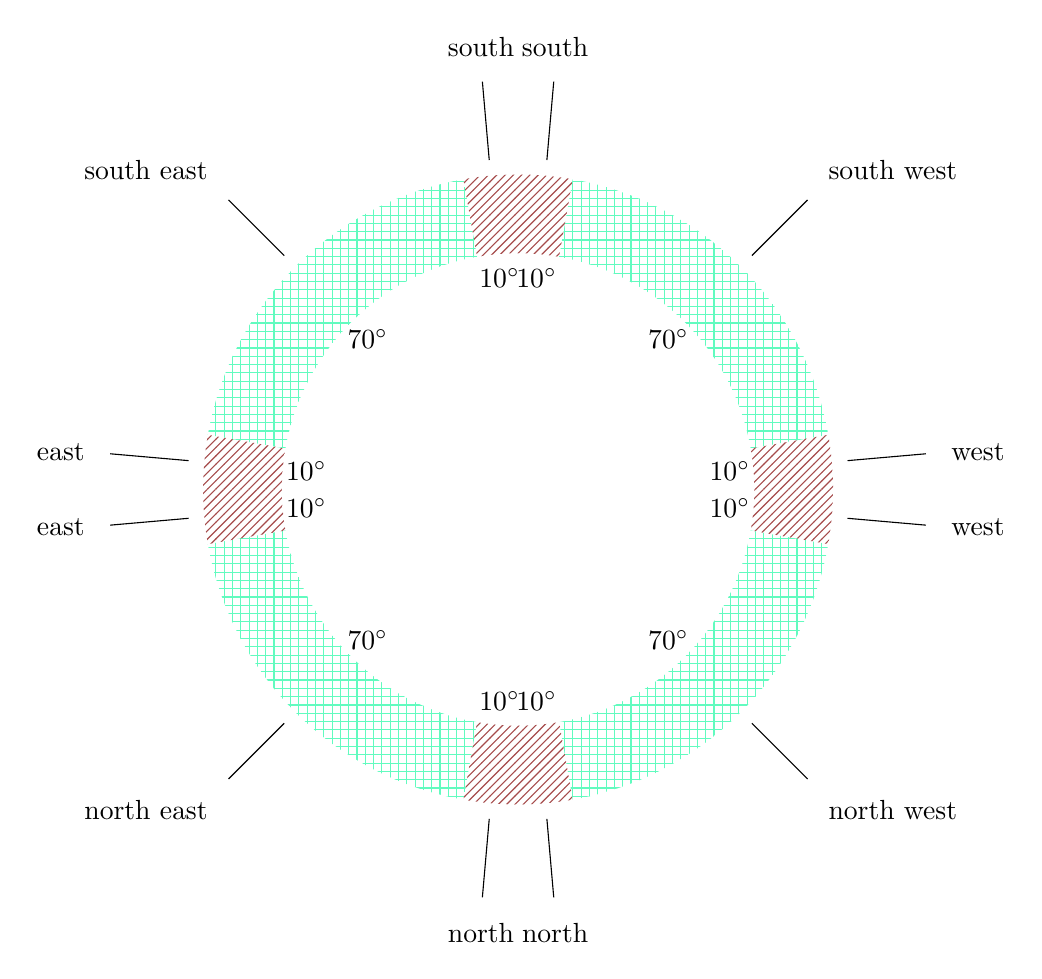
\begin{tikzpicture}
\wheelchart[
    inner data={$\WCvarA^{\circ}$},
    %inner data style={shift={(\WCmidangle:{-0.1})}},
    inner data sep=0.3,
    lines,
    radius={3}{4},
    slices style={pattern=\WCvarD,pattern color=\WCvarB!70},
]{%
    10/Maroon/south/{north east lines},
    70/TealBlue/{south west}/grid,
    10/Maroon/west/{north east lines},
    10/Maroon/west/{north east lines},
    70/TealBlue/{north west}/grid,
    10/Maroon/north/{north east lines},
    10/Maroon/north/{north east lines},
    70/TealBlue/{north east}/grid,
    10/Maroon/east/{north east lines},
    10/Maroon/east/{north east lines},
    70/TealBlue/{south east}/grid,
    10/Maroon/south/{north east lines}%
}
\end{tikzpicture}
\end{codeexample}
\begin{codeexample}[width=10cm,preamble={\usetikzlibrary{patterns}}]
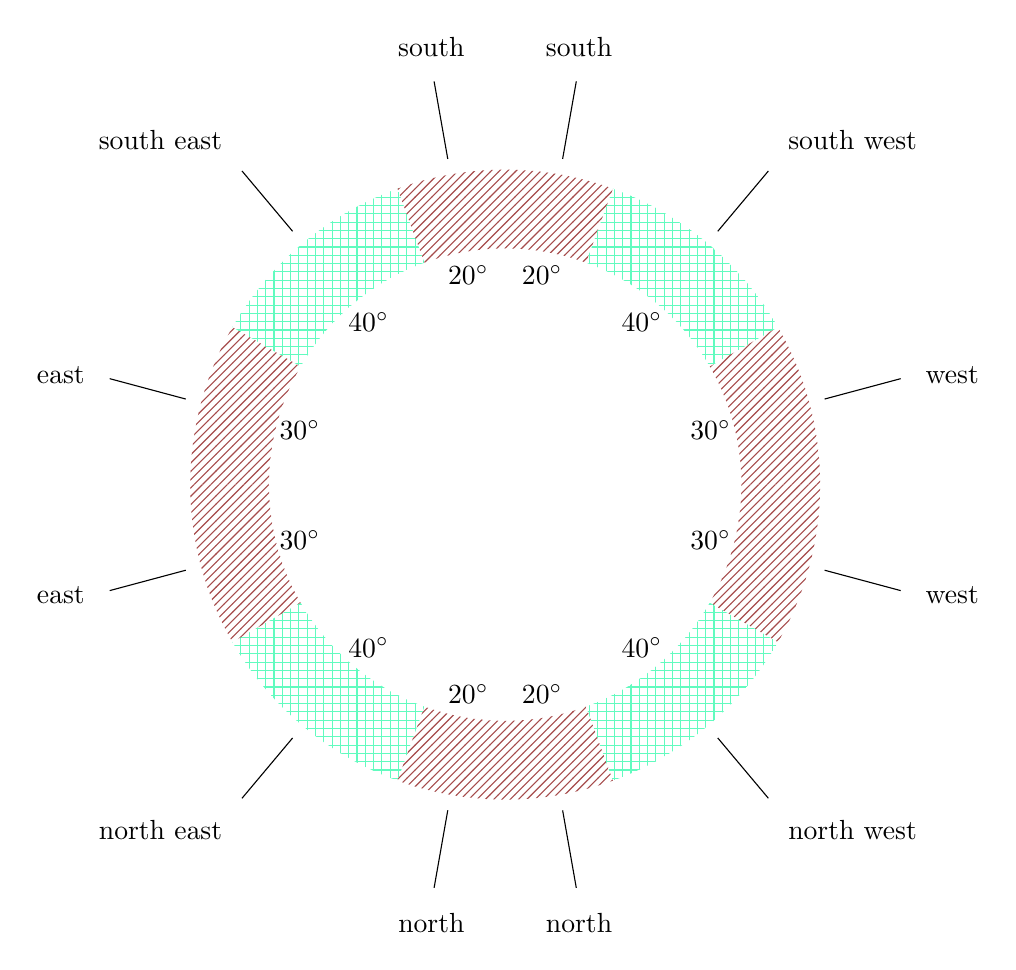
\begin{tikzpicture}
\wheelchart[
    anchor xsep=10,
    anchor ysep=15,
    inner data={$\WCvarA^{\circ}$},
    %inner data style={shift={(\WCmidangle:{-0.1})}},
    inner data sep=0.3,
    lines,
    radius={3}{4},
    slices style={pattern=\WCvarD,pattern color=\WCvarB!70},
]{%
    20/Maroon/south/{north east lines},
    40/TealBlue/{south west}/grid,
    30/Maroon/west/{north east lines},
    30/Maroon/west/{north east lines},
    40/TealBlue/{north west}/grid,
    20/Maroon/north/{north east lines},
    20/Maroon/north/{north east lines},
    40/TealBlue/{north east}/grid,
    30/Maroon/east/{north east lines},
    30/Maroon/east/{north east lines},
    40/TealBlue/{south east}/grid,
    20/Maroon/south/{north east lines}%
}
\end{tikzpicture}
\end{codeexample}
The anchor of the key |data| can also be specified manually by using the key |data style|.
\begin{codeexample}[width=10cm,preamble={\usetikzlibrary{patterns}}]
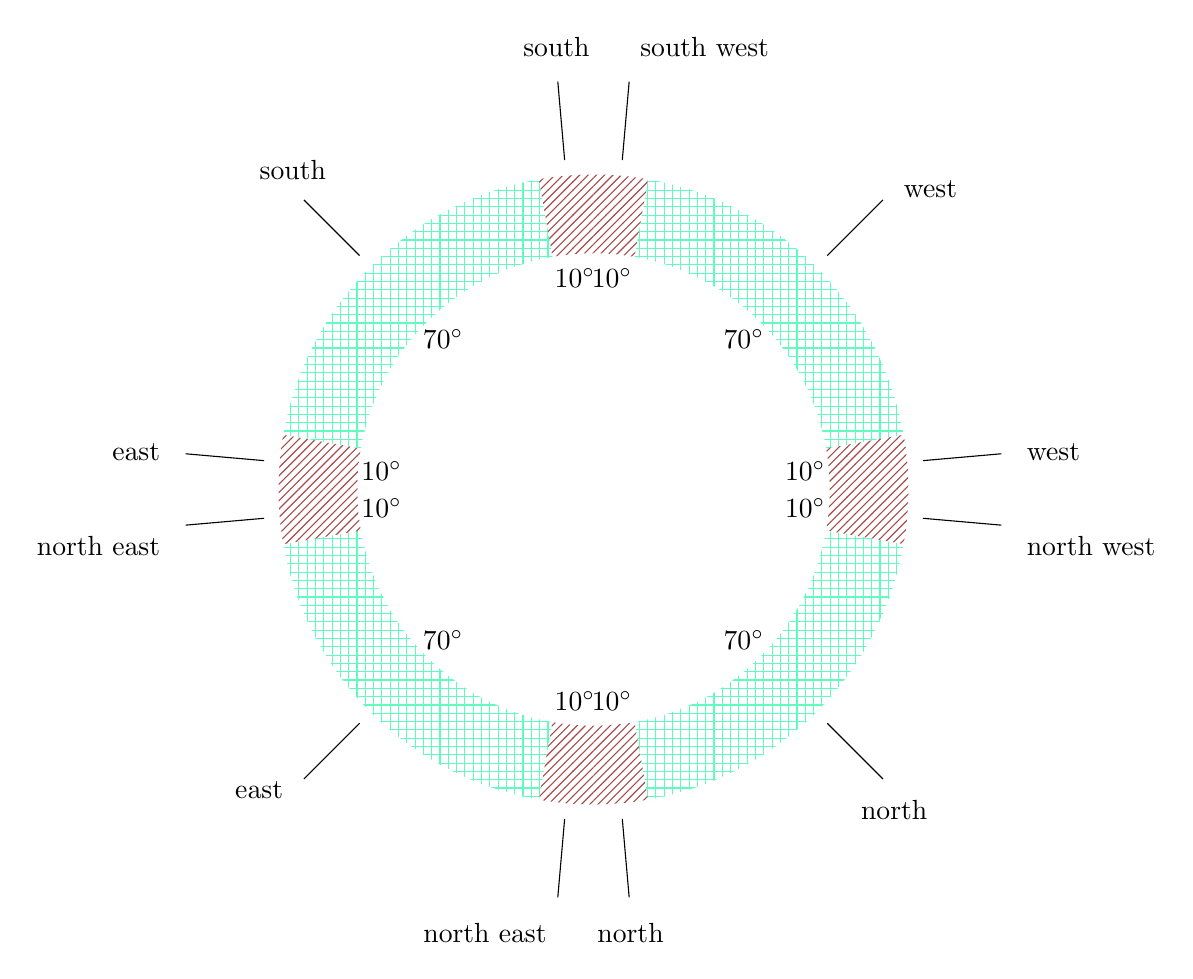
\begin{tikzpicture}
\wheelchart[
    data style={anchor=\WCvarC},
    inner data={$\WCvarA^{\circ}$},
    %inner data style={shift={(\WCmidangle:{-0.1})}},
    inner data sep=0.3,
    lines,
    radius={3}{4},
    slices style={pattern=\WCvarD,pattern color=\WCvarB!70},
]{%
    10/Maroon/{south west}/{north east lines},
    70/TealBlue/west/grid,
    10/Maroon/west/{north east lines},
    10/Maroon/{north west}/{north east lines},
    70/TealBlue/north/grid,
    10/Maroon/north/{north east lines},
    10/Maroon/{north east}/{north east lines},
    70/TealBlue/east/grid,
    10/Maroon/{north east}/{north east lines},
    10/Maroon/east/{north east lines},
    70/TealBlue/south/grid,
    10/Maroon/south/{north east lines}%
}
\end{tikzpicture}
\end{codeexample}
\end{key}
\begin{key}{/wheelchart/at=\marg{point} (initially (0,0))}
This key defines the center of the wheelchart.
\end{key}
\begin{key}{/wheelchart/caption=\marg{text}}
This key contains the \meta{text} which will be placed below the wheelchart. The \meta{text} is placed in a node. The $x$ coordinate of this node is the $x$ coordinate of the center of the wheelchart, which is defined by the key |at|. In general, this is \emph{not} the same as the $x$ coordinate of the center of the |local bounding box| around the wheelchart. The $y$ coordinate of this node is |0.5| below the south of the |local bounding box| around the wheelchart. The style of this node is given as follows. First, the options |anchor=north,align=center| are given. Thereafter, the style of the key |caption style| is added.
\end{key}
\begin{key}{/wheelchart/caption left=\marg{text}}
This key contains the \meta{text} which will be placed below left of the wheelchart. The \meta{text} is placed in a node. This node is placed |0.5| below the south west of the |local bounding box| around the wheelchart. The style of this node is given as follows. First, the options |anchor=north west,align=left| are given. Thereafter, the style of the key |caption left style| is added.
\end{key}
\begin{stylekey}{/wheelchart/caption left style=\marg{options} (initially \normalfont empty)}
This key accepts a list of keys which will be applied to the node where the contents of the key |caption left| is placed.
\end{stylekey}
\begin{stylekey}{/wheelchart/caption style=\marg{options} (initially \normalfont empty)}
This key accepts a list of keys which will be applied to the node where the contents of the key |caption| is placed.
\begin{codeexample}[width=10cm]
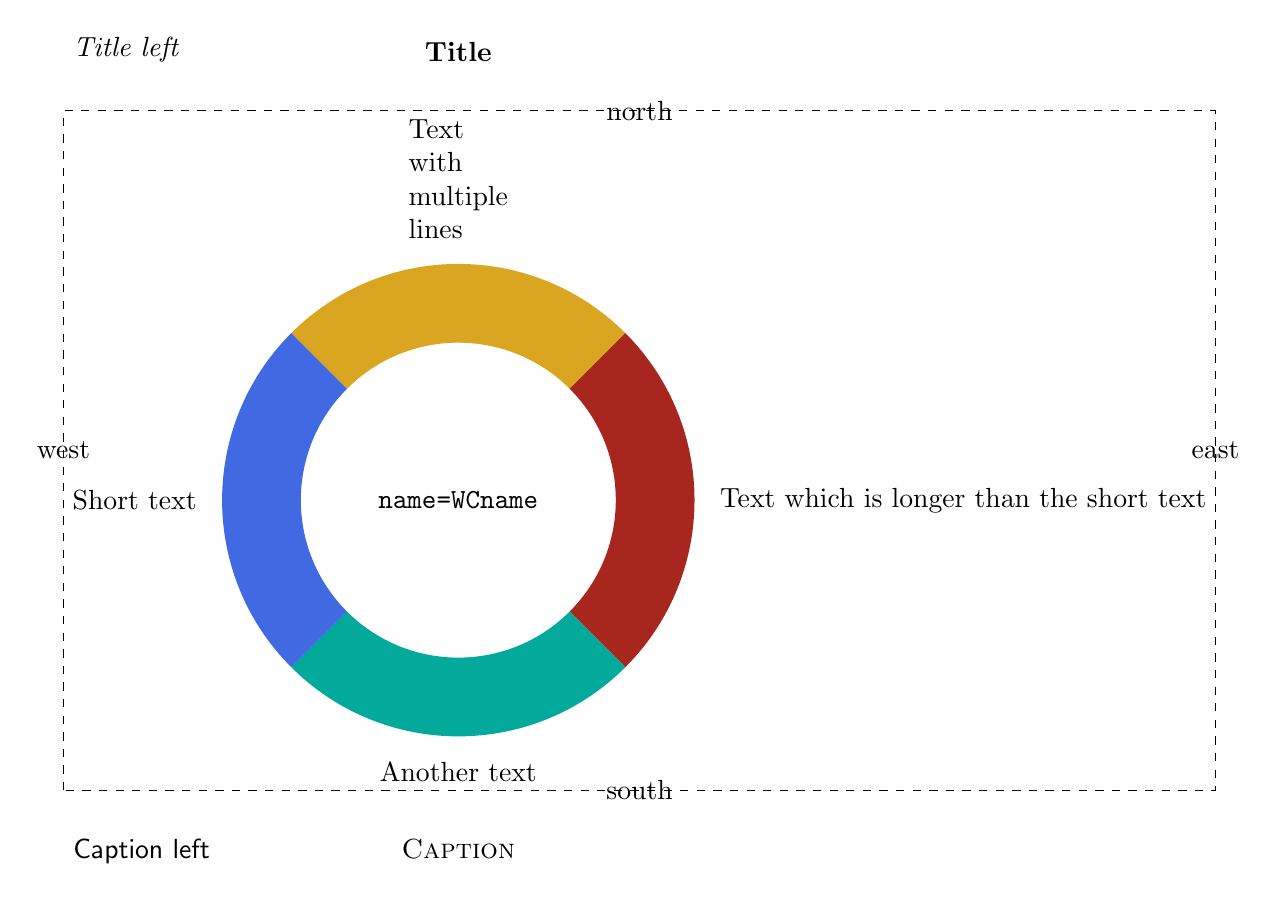
\begin{tikzpicture}
\wheelchart[
    at={(5,2)},
    caption=Caption,
    caption style={font=\scshape},
    caption left={Caption left},
    caption left style={font=\sffamily},
    middle={\texttt{name=WCname}},
    name=WCname,
    start half,
    title=Title,
    title style={font=\bfseries},
    title left={Title left},
    title left style={font=\em}
]{%
    1/Goldenrod/{Text\\with\\multiple\\lines},
    1/Mahogany/{Text which is longer than the short text},
    1/JungleGreen/{Another text},
    1/RoyalBlue/{Short text}%
}
\draw[dashed] (WCname.south west) rectangle (WCname.north east);
\foreach\pos in {north,east,south,west}{
    \node at (WCname.\pos) {\pos};
}
\end{tikzpicture}
\end{codeexample}
\end{stylekey}
\begin{stylekey}{/wheelchart/contour=\marg{options} (initially \normalfont empty)}
If this key is set then a contour with the style determined by this key will be drawn around the wheelchart.
\end{stylekey}
\begin{key}{/wheelchart/counterclockwise=\opt{\meta{boolean}} (default true, initially false)}
If true, the wheelchart will be drawn counterclockwise instead of clockwise.
\begin{codeexample}[width=10cm]
\begin{tikzpicture}
\wheelchart[
    counterclockwise,
    middle=counterclockwise,
    middle style={font=\ttfamily}
]{\exampleforthismanual}
\end{tikzpicture}
\end{codeexample}
\end{key}
\begin{key}{/wheelchart/data=\marg{text} (initially \textbackslash WCvarC)}
This key contains the \meta{text} which will be placed at the outside of each slice of the wheelchart. This can be suppressed by using |data={}|. The \meta{text} is placed in a node. The style of this node is given as follows. First, the anchor is set following Table \ref{tableanchorofthekeydatainthecasethatlinesextequaltozero} and Table \ref{tableanchorofthekeydatainthecasethatlinesextstrictlylargerthanzero}. Then the option |align=left| is added. Thereafter, the style of the key |data style| is added.
\end{key}
\begin{key}{/wheelchart/data angle shift=\marg{angle} (initially 0)}
The contents of the key |data| is placed at the angle |\WCdataangle|, which is the sum of the value of the key |data angle shift| in degrees (taking into account the key |counterclockwise|) and the macro |\WCmidangle| modulo $360$.
\end{key}
\begin{key}{/wheelchart/data sep=\marg{value} (initially 0.2)}
If |lines=0|, this key defines the distance between the wheelchart and the contents of the key |data|. If $\text{|lines|}>0$, this key defines the distance between the end of the lines and the contents of the key |data|.
\end{key}
\begin{stylekey}{/wheelchart/data style=\marg{options} (initially \normalfont empty)}
This key accepts a list of keys which will be applied to the node where the contents of the key |data| is placed.
\end{stylekey}
\begin{key}{/wheelchart/expand list=\mchoice{false,once,true} (initially once)}
\begin{description}
\item[\texttt{false}] In this case, the \meta{wheelchart data} of the command |\wheelchart| will not be expanded.
\item[\texttt{once}] In this case, the \meta{wheelchart data} of the command |\wheelchart| will be expanded once.
\item[\texttt{true}] In this case, the \meta{wheelchart data} of the command |\wheelchart| will be fully expanded.
\end{description}
The following example illustrates the difference between the possible values of the key |expand list|.
\begin{codeexample}[width=10cm,preamble={\usepackage{listofitems}}]
\readlist*\WCcolors{
    Dandelion,CarnationPink,
    SpringGreen,ProcessBlue
}
\begin{tikzpicture}
\def\WClistA{a,A}
\def\WClistB{b,B}
\def\WCdata{\WClistA,\WClistB}
\foreach\expandlist [count=\n] in
    {false,once,true}{
\wheelchart[
    at={({3.5*\n},0)},
    data=\WCvarA,
    expand list=\expandlist,
    radius={0}{1},
    slices style={\WCcolors[\WCcount]},
    title={expand list=\\\expandlist},
    title style={font=\ttfamily},
    value=1
]{\WCdata}
}
\end{tikzpicture}
\end{codeexample}
The initial setting |expand list=once| works in most situations, even when commands such as |\ref|, |\cite| and |\textbf| are used such as in the example below.
\begin{codeexample}[width=10cm]
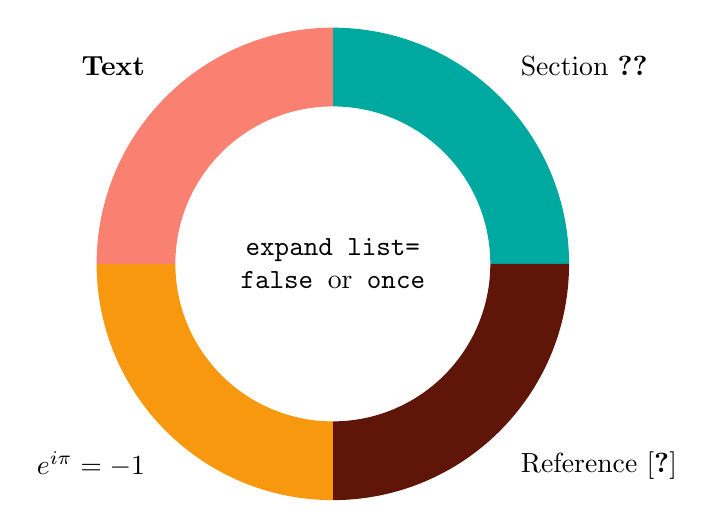
\begin{tikzpicture}
\wheelchart[
    %expand list=false,%false also works
    %expand list=true,%true doesn't work
    middle={expand list=\\false %
        {\normalfont or} once},
    middle style={font=\ttfamily}
]{%
    1/Emerald/{Section \ref{Keys}},
    1/Sepia/{Reference \cite{TtTaPGFp}},
    1/YellowOrange/{$e^{i\pi}=-1$},
    1/Salmon/{\textbf{Text}}%
}
\end{tikzpicture}
\end{codeexample}
In the following example, the \meta{wheelchart data} from the previous example is stored in a macro. In this case, we have to use the initial setting |expand list=once|.
\begin{codeexample}[width=10cm]
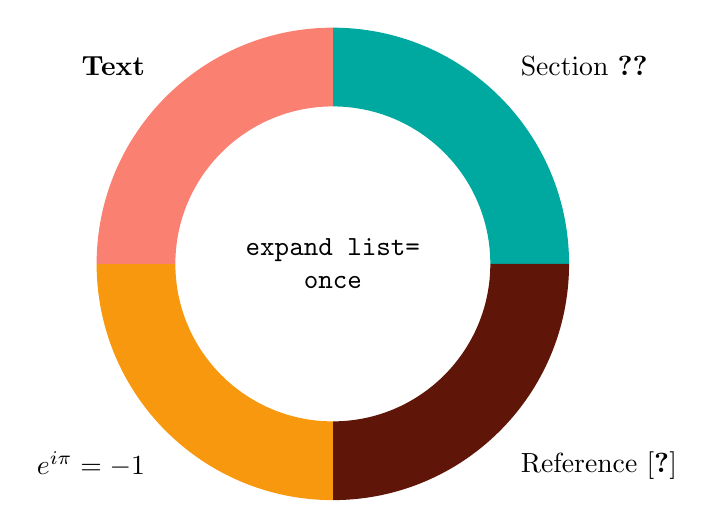
\begin{tikzpicture}
\def\WClist{%
    1/Emerald/{Section \ref{Keys}},
    1/Sepia/{Reference \cite{TtTaPGFp}},
    1/YellowOrange/{$e^{i\pi}=-1$},
    1/Salmon/{\textbf{Text}}%
}
\wheelchart[
    %expand list=false,
    %expand list=true,
    %false and true do not work
    middle={expand list=\\once},
    middle style={font=\ttfamily}
]{\WClist}
\end{tikzpicture}
\end{codeexample}
In the example below, we have to use |expand list=true|.
\begin{codeexample}[width=10cm]
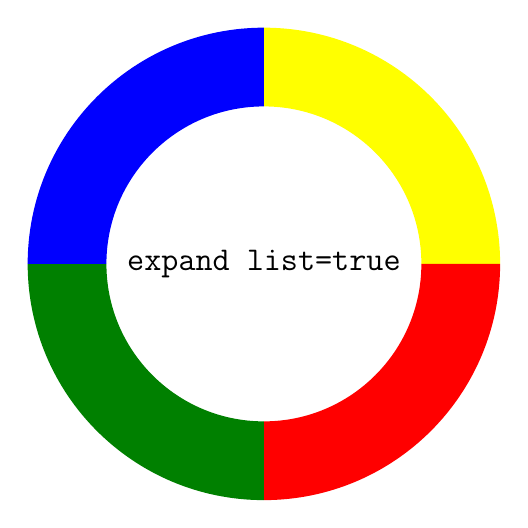
\begin{tikzpicture}
\def\WCcolorsA{Yellow,Red}
\def\WCcolorsB{Green,Blue}
\wheelchart[
    data={},
    expand list=true,%false and once
                     %do not work
    middle={expand list=true},
    middle style={font=\large\ttfamily},
    slices style={\WCvarA},
    value=1
]{\WCcolorsA,\WCcolorsB}
\end{tikzpicture}
\end{codeexample}
In the example below, we have to use |expand list=true| and the command |\expandonce| from the package |etoolbox|.
\begin{codeexample}[width=10cm,preamble={\usepackage{etoolbox}}]
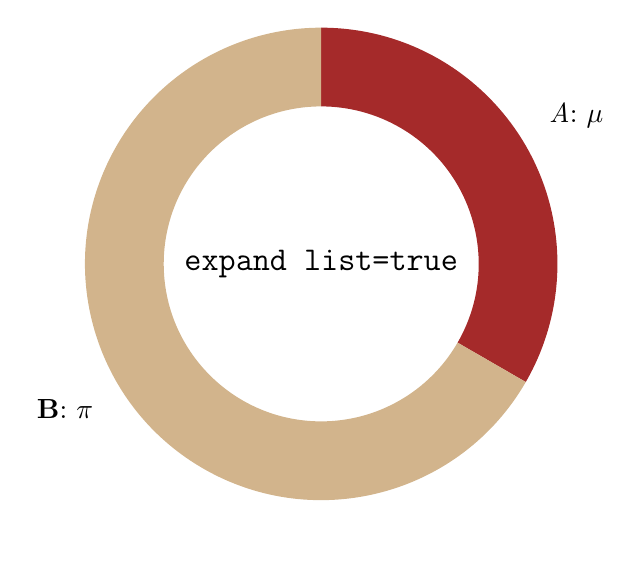
\begin{tikzpicture}
\def\WCsliceA{1/Brown/{\emph{A}: $\mu$}}
\def\WCsliceAfinal{\expandonce\WCsliceA}
\def\WCsliceB{2/Tan/{\textbf{B}: $\pi$}}
\def\WCsliceBfinal{\expandonce\WCsliceB}
\wheelchart[
    expand list=true,%false and once
                     %do not work
    middle={expand list=true},
    middle style={font=\large\ttfamily},
]{\WCsliceAfinal,\WCsliceBfinal}
%\WCsliceA and \WCsliceB do not work
\end{tikzpicture}
\end{codeexample}
\end{key}
\begin{key}{/wheelchart/explode=\marg{value} (default 0.2, initially 0)}
This key will shift the slices of the wheelchart with \meta{value} with respect to the center of the wheelchart.
\begin{codeexample}[width=10cm]
\begin{tikzpicture}
\wheelchart[
    explode=\WCvarF,
    pie
]{\exampleforthismanual}
\end{tikzpicture}
\end{codeexample}
\end{key}
\begin{key}{/wheelchart/gap=\marg{value} (default 0.05, initially 0)}
The \meta{value} of this key defines half the distance between two slices of the wheelchart.

The following example illustrates the behaviour of the key |gap| when a slice has $360$ degrees.
\begin{codeexample}[width=10cm]
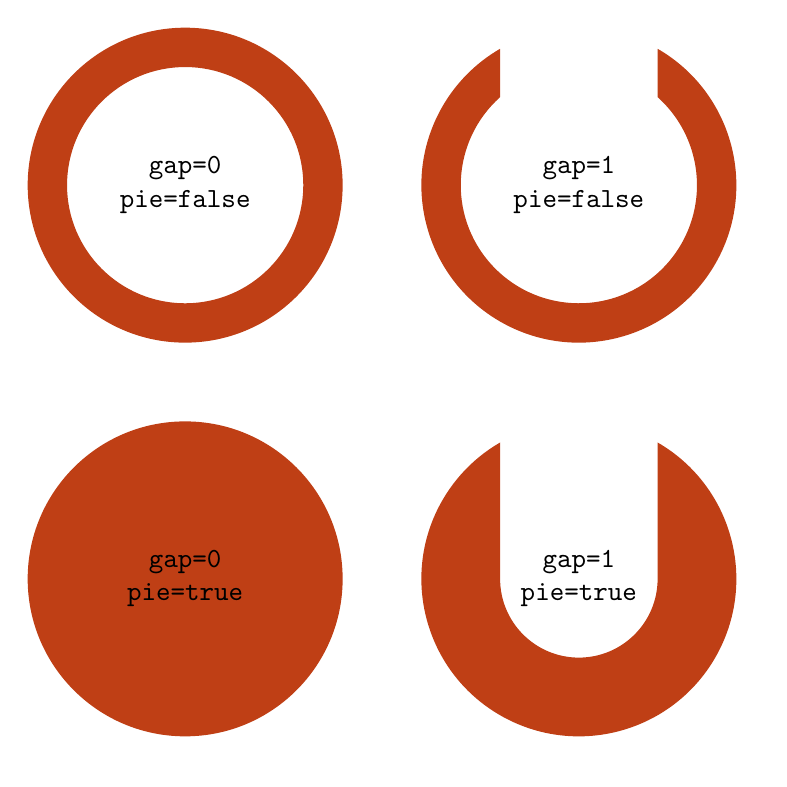
\begin{tikzpicture}
\foreach\gap [count=\m] in {0,1}{
\foreach\pie [count=\n] in {false,true}{
\wheelchart[
    at={({5*\m},{-5*\n})},
    data={},
    gap=\gap,
    middle={gap=\gap\\pie=\pie},
    middle style={font=\ttfamily},
    pie=\pie,
    radius={1.5}{2},
    slices style=Bittersweet,
    total count=1,
    value=1
]{}
}
}
\end{tikzpicture}
\end{codeexample}
\end{key}
\begin{key}{/wheelchart/gap polar=\marg{value} (default 1, initially 0)}
The \meta{value} of this key defines half the polar gap in degrees between two slices of the wheelchart.

Note the difference between the keys |explode|, |gap| and |gap polar|. This is illustrated in the examples below.
\begin{codeexample}[width=10cm]
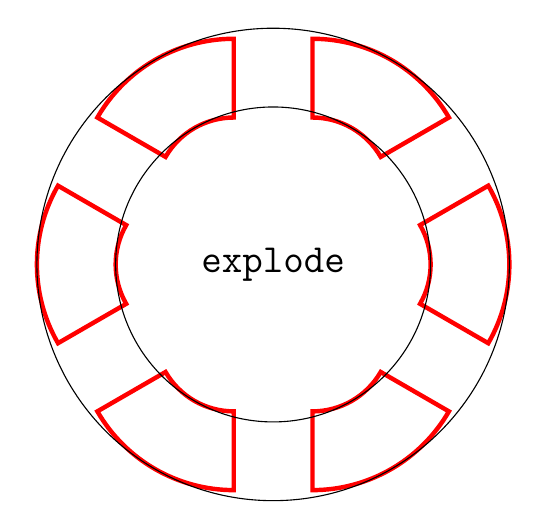
\begin{tikzpicture}
\wheelchart[
    data={},
    explode=1,
    middle={\Large\texttt{explode}},
    radius={1}{2},
    slices style={
        draw=Red,
        fill=none,
        ultra thick
    },
    total count=6,
    value=1
]{}
\draw (0,0) circle[radius=2];
\draw (0,0) circle[radius=3];
\end{tikzpicture}
\end{codeexample}
\begin{codeexample}[width=10cm]
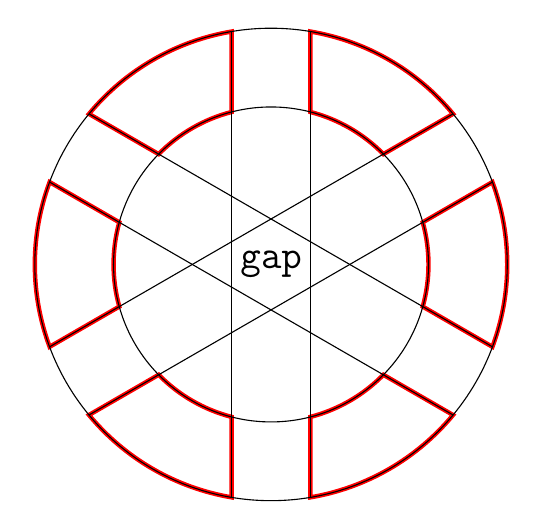
\begin{tikzpicture}
\wheelchart[
    data={},
    gap=0.5,
    middle={\Large\texttt{gap}},
    slices style={
        draw=Red,
        fill=none,
        ultra thick
    },
    total count=6,
    value=1
]{}
\draw (0,0) circle[radius=2];
\draw (0,0) circle[radius=3];
\foreach\a in {0,60,120}{
\foreach\x in {-0.5,0.5}{
\draw[rotate=\a] (\x,{sqrt(3^2-0.5^2})--
    (\x,{-sqrt(3^2-0.5^2});
}
}
\end{tikzpicture}
\end{codeexample}
\begin{codeexample}[width=10cm]
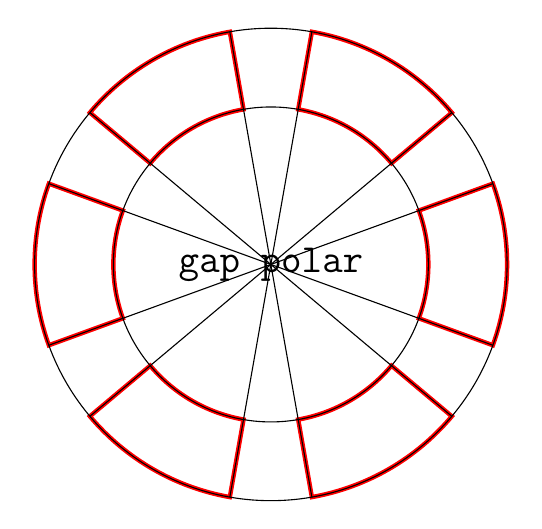
\begin{tikzpicture}
\wheelchart[
    data={},
    gap polar=10,
    middle={\Large\texttt{gap polar}},
    slices style={
        draw=Red,
        fill=none,
        ultra thick
    },
    total count=6,
    value=1
]{}
\draw (0,0) circle[radius=2];
\draw (0,0) circle[radius=3];
\foreach\a in {30,90,150}{
\foreach\t in {-10,10}{
\draw ({\t+\a}:3)--({\t+\a+180}:3);
}
}
\end{tikzpicture}
\end{codeexample}
\end{key}
\begin{key}{/wheelchart/inner data=\marg{text}}
This key contains the \meta{text} which will be placed at the inside of each slice of the wheelchart. The \meta{text} is placed in a node. The style of this node is given as follows. First, the option |align=left| is given. Thereafter, the style of the key |inner data style| is added.
\end{key}
\begin{key}{/wheelchart/inner data sep=\marg{value} (initially 0.2)}
This key defines the distance between the wheelchart and the contents of the key |inner data|.
\end{key}
\begin{stylekey}{/wheelchart/inner data style=\marg{options} (initially \normalfont empty)}
This key accepts a list of keys which will be applied to the node where the contents of the key |inner data| is placed.
\end{stylekey}
\begin{key}{/wheelchart/inner radius=\marg{value} (initially 2)}
The \meta{value} of this key defines the inner radius of the wheelchart.
\end{key}
\begin{key}{/wheelchart/legend=\marg{code}}
If this key is set then the \meta{code} given to this key will be executed at the end of the command |\wheelchart|.
\end{key}
\begin{key}{/wheelchart/legend entry=\marg{code}}
If this key is set then the \meta{code} given to this key will be executed for each slice of the wheelchart.
\begin{codeexample}[width=10cm,preamble={\usepackage{etoolbox}}]
\begin{tikzpicture}
\def\WClegend{}
\def\WClegendrow#1#2#3#4#5{\tikz\fill[#1] (0,0) rectangle (0.3,0.3); & #2 & $#3$ & #4 & #5\\}
\wheelchart[
    data={},
    legend entry={
        \gappto\WClegend{\WClegendrow}
        \xappto\WClegend{{\WCvarB}{\WCvarC}{\WCvarA}{\WCperc}{\WCvarD}}
    },
    legend={
        \node[anchor=west] at (3.5,0) {%
            \begin{tabular}{l@{ }lrrl}%
             & Fruit & Value & Percentage & Vitamines\\\hline%
            \\[-10pt]%
            \WClegend\hline%
             & \textbf{Total} & $\pgfmathprintnumber{\WCtotalnum}$ & & \\%
            \end{tabular}%
        };
    }
]{\exampleforthismanual}
\end{tikzpicture}
\end{codeexample}
\end{key}
\begin{key}{/wheelchart/lines=\marg{value} (default 1, initially 0)}
This key will draw lines of length \meta{value} between the wheelchart and the contents of the key |data|.
\begin{codeexample}[width=10cm]
\begin{tikzpicture}
\def\WCtest#1#2{%
    \ifdim \WCpercentage pt>10 pt%
        #1%
    \else%
        #2%
    \fi%
}
\wheelchart[
    data={\WCtest{}{\WCperc}},
    lines={
        1-max(sign(\WCpercentage-10),0)
    },
    lines style={dotted,thick},
    pie,
    wheel data={\WCtest{\WCperc}{}}
]{\exampleforthismanual}
\end{tikzpicture}
\end{codeexample}
\end{key}
\begin{key}{/wheelchart/lines ext=\marg{value} (default 0.5, initially 0)}
If the \meta{value} of this key is $>0$ then the lines between the wheelchart and the contents of the key |data| will be extended horizontally with a length defined by 	\meta{value}.
\end{key}
\begin{key}{/wheelchart/lines ext bottom dir=\mchoice{left,right} (initially right)}
This key applies when |\WCdataangle|${}\in[270-\text{|lines ext dirsep|},270+\text{|lines ext dirsep|}]$. In this case, this key defines the direction in which the lines between the wheelchart and the contents of the key |data| will be extended horizontally and in this case, this key also determines the anchor of the key |data|.
\begin{description}
\item[\texttt{left}] In this case, the lines between the wheelchart and the contents of the key |data| will be extended horizontally to the left and the anchor of the key |data| is the value of the key |lines ext left anchor|.
\item[\texttt{right}] In this case, the lines between the wheelchart and the contents of the key |data| will be extended horizontally to the right and the anchor of the key |data| is the value of the key |lines ext right anchor|.
\end{description}
\end{key}
\begin{key}{/wheelchart/lines ext dirsep=\marg{angle} (initially 0)}
This key determines half the angle in degrees of the segment to which the keys |lines ext bottom dir| and |lines ext top dir| apply.
\end{key}
\begin{key}{/wheelchart/lines ext fixed=\opt{\meta{boolean}} (default true, initially false)}
If true, all lines between the wheelchart and the contents of the key |data| will be extended horizontally till the same $x$ coordinate at the left and till the same $x$ coordinate at the right.
\end{key}
\begin{key}{/wheelchart/lines ext left anchor=\marg{anchor} (initially mid east)}
This key defines the anchor of the key |data| when the lines between the wheelchart and the contents of the key |data| are extended horizontally to the left.
\end{key}
\begin{key}{/wheelchart/lines ext right anchor=\marg{anchor} (initially mid west)}
This key defines the anchor of the key |data| when the lines between the wheelchart and the contents of the key |data| are extended horizontally to the right.
\end{key}
\begin{key}{/wheelchart/lines ext top dir=\mchoice{left,right} (initially right)}
This key applies when |\WCdataangle|${}\in[90-\text{|lines ext dirsep|},90+\text{|lines ext dirsep|}]$. In this case, this key defines the direction in which the lines between the wheelchart and the contents of the key |data| will be extended horizontally and in this case, this key also determines the anchor of the key |data|.
\begin{description}
\item[\texttt{left}] In this case, the lines between the wheelchart and the contents of the key |data| will be extended horizontally to the left and the anchor of the key |data| is the value of the key |lines ext left anchor|.
\item[\texttt{right}] In this case, the lines between the wheelchart and the contents of the key |data| will be extended horizontally to the right and the anchor of the key |data| is the value of the key |lines ext right anchor|.
\end{description}
\begin{table}[ht]
\centering
\begin{tabular}{ll}
 & Anchor of the key |data|\\
|\WCdataangle| & in the case that $\text{|lines ext|}>0$\\\hline
$\rinterval{0}{90-\text{|lines ext dirsep|}}$ & value of the key |lines ext right anchor|\\
$[90-\text{|lines ext dirsep|},90+\text{|lines ext dirsep|}]$ & value of the key |lines ext left anchor|\\
 & if |lines ext top dir=left|\\
 & value of the key |lines ext right anchor|\\
 & if |lines ext top dir=right|\\
$\ointerval{90+\text{|lines ext dirsep|}}{270-\text{|lines ext dirsep|}}$ & value of the key |lines ext left anchor|\\
$[270-\text{|lines ext dirsep|},270+\text{|lines ext dirsep|}]$ & value of the key |lines ext left anchor|\\
 & if |lines ext bottom dir=left|\\
 & value of the key |lines ext right anchor|\\
 & if |lines ext bottom dir=right|\\
$\ointerval{270+\text{|lines ext dirsep|}}{360}$ & value of the key |lines ext right anchor|\\
\end{tabular}
\caption{Anchor of the key \texttt{data} in the case that $\text{\ttfamily lines ext}>0$.}\label{tableanchorofthekeydatainthecasethatlinesextstrictlylargerthanzero}
\end{table}
The number of columns in the legend in the example below can be specified with |\WClegendcolumns|.
\begin{codeexample}[width=10cm,preamble={\usepackage{etoolbox}
\usetikzlibrary{decorations.markings}}]
\begin{tikzpicture}
\def\WClegendcolumns{2}%specify the number of columns in the legend
\def\WClegendrow#1#2#3{\tikz\fill[#1] (0,0) circle[radius=0.15]; & #2 & $#3$}
\wheelchart[
    data={\WCperc},
    data style={outer xsep=4pt},
    legend entry={
        \csgdef{WClegend\WCcount}{}
        \csgappto{WClegend\WCcount}{\WClegendrow}
        \csxappto{WClegend\WCcount}{{\WCvarB}{\WCvarC}{\WCvarA}}
    },
    legend={
        \def\WClegend{}
        \pgfmathsetmacro{\WClegendrows}{int(ceil(\WCtotalcount/\WClegendcolumns))}
        \foreach\n in {1,...,\WClegendrows}{
            \foreach\k in {1,...,\WClegendcolumns}{
                \pgfmathparse{int(\n+(\k-1)*\WClegendrows)}
                \ifnum\pgfmathresult>\WCtotalcount
                    \gappto\WClegend{ & & }
                \else
                    \gappto\WClegend{\csname WClegend}
                    \xappto\WClegend{\pgfmathresult}
                    \gappto\WClegend{\endcsname}
                \fi
                \ifnum\k=\WClegendcolumns
                    \gappto\WClegend{\\}
                \else
                    \gappto\WClegend{ & }
                \fi
            }
        }
        \node[anchor=north,draw,rounded corners,thick] at (0,-4.5) {%
            \begin{tabular}{*{\WClegendcolumns}{l@{ }lr}}%
            \WClegend%
            \end{tabular}%
        };
    },
    lines=0.5,
    lines ext=1,
    lines ext bottom dir=left,
    lines ext dirsep=1,
    lines ext fixed,
    lines ext top dir=right,
    lines sep=0,
    lines style={
        \WCvarB,
        postaction=decorate,
        decoration={
            markings,
            mark=at position 1 with {
                \fill[\WCvarB] (0,0) circle[radius=0.15];
            }
        }
    },
    start angle=331.2
]{\exampleforthismanual}
\wheelchart[
    data={},
    radius={1.5}{2},
    slices style=\WCvarB!70,
    start angle=331.2
]{\exampleforthismanual}
\end{tikzpicture}
\end{codeexample}
\begin{codeexample}[width=10cm]
\begin{tikzpicture}
\wheelchart[
    data style={
        inner sep=0pt,
        shift={(0,0.1)}
    },
    lines,
    lines ext=1.2,
    lines ext bottom dir=right,
    lines ext dirsep=1,
    %lines ext fixed,
    lines ext left anchor={base west},
    lines ext right anchor={base east},
    lines ext top dir=left,
    lines sep=-0.5,
    %lines style=\WCvarB,
    start angle=331.2
]{\exampleforthismanual}
\end{tikzpicture}
\end{codeexample}
\begin{codeexample}[width=10cm,preamble={\usetikzlibrary{decorations.markings}}]
\begin{tikzpicture}
\wheelchart[
    data={\WCvarC: \WCvarA},
    data angle shift=\WCvarG,
    data style={draw=\WCvarB,fill=\WCvarB!20},
    lines=1.5,
    lines ext=1,
    lines sep=-1,
    lines style={
        Black,
        postaction=decorate,
        decoration={
            markings,
            mark=at position 0 with {
                \fill[Black] (0,0) circle[radius=0.15];
            }
        }
    },
    pie,
    start angle=331.2
]{\exampleforthismanual}
\end{tikzpicture}
\end{codeexample}
\end{key}
\begin{key}{/wheelchart/lines sep=\marg{value} (initially 0.2)}
This key defines the distance between the wheelchart and the start of the lines.
\end{key}
\begin{stylekey}{/wheelchart/lines style=\marg{options} (initially \normalfont empty)}
This key accepts a list of keys which will be applied to the lines drawn by the key |lines|.
\end{stylekey}
\begin{key}{/wheelchart/middle=\marg{text}}
This key contains the \meta{text} which will be placed at the center of the wheelchart. The \meta{text} is placed in a node. The style of this node is given as follows. First, the option |align=center| is given. Thereafter, the style of the key |middle style| is added.
\end{key}
\begin{stylekey}{/wheelchart/middle fill=\marg{options} (initially \normalfont empty)}
If this key is set then the middle of the wheelchart will be filled with this style.
\begin{codeexample}[width=10cm]

\begin{tikzpicture}
\wheelchart[
    counterclockwise,
    data={},
    middle fill={
        Green,
        draw=Red,
        ultra thick
    },
    radius={0.8*\WCcount}
        {0.4+0.8*\WCcount},
    slices style={
        draw=Blue,
        fill=none,
        ultra thick
    },
    start angle=0,
    total angle=300,
    total count=4,
    value=1
]{}
\end{tikzpicture}
\end{codeexample}
\end{stylekey}
\begin{stylekey}{/wheelchart/middle style=\marg{options} (initially \normalfont empty)}
This key accepts a list of keys which will be applied to the node where the contents of the key |middle| is placed.
\end{stylekey}
\begin{key}{/wheelchart/name=\marg{name} (initially wheelchart@name)}
This key defines the \meta{name} of the |local bounding box| around the wheelchart.
\end{key}
\begin{key}{/wheelchart/outer radius=\marg{value} (initially 3)}
The \meta{value} of this key defines the outer radius of the wheelchart.
\end{key}
\begin{key}{/wheelchart/perc precision=\marg{number} (initially 0)}
This key defines the number of decimals up to which the percentage in the macros |\WCperc| and |\WCpercentagerounded| are rounded.
\end{key}
\begin{key}{/wheelchart/pie=\opt{\meta{boolean}} (default true, initially false)}
If true, the inner radius of the wheelchart is set to |0|.
\end{key}
\begin{key}{/wheelchart/radius=\marg{inner radius}\marg{outer radius}}
This key defines the inner and outer radius of the wheelchart.
\begin{codeexample}[width=10cm]
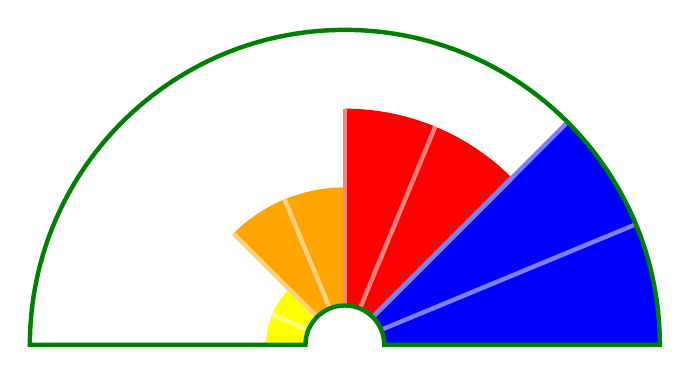
\begin{tikzpicture}
\wheelchart[
    contour={Green,ultra thick},
    data={},
    radius={0.5}{\WCcount},
    slices style=\WCvarA,
    start angle=180,
    total angle=180,
    value=2,
    wheel lines={\WCvarA!50,ultra thick}
]{Yellow,Orange,Red,Blue}
\end{tikzpicture}
\end{codeexample}
\begin{codeexample}[width=10cm,preamble={\usepackage{siunitx}}]
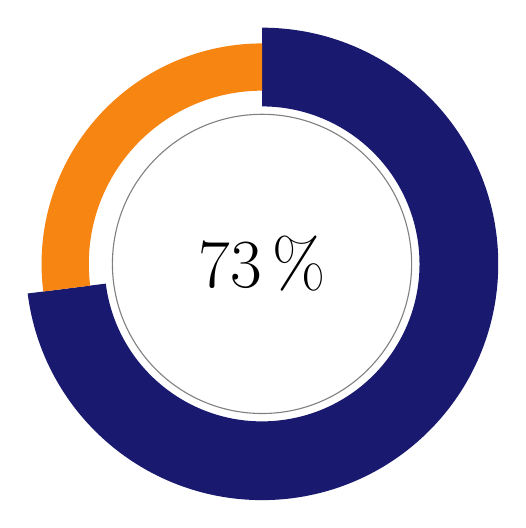
\begin{tikzpicture}
\def\n{73}
\wheelchart[
    data={},
    middle={{\Huge\qty{\n}{\percent}}},
    radius={2.5-\WCvarC}{2.5+\WCvarC}
]{%
    \n/MidnightBlue/0.5,
    {100-\n}/BurntOrange/0.3%
}
\draw[Gray] (0,0) circle[radius=1.9];
\end{tikzpicture}
\end{codeexample}
\end{key}
\begin{key}{/wheelchart/slices=\marg{path}}
If this key is set then the shape of the slices of the wheelchart is defined by \meta{path}.
\begin{codeexample}[width=10cm]
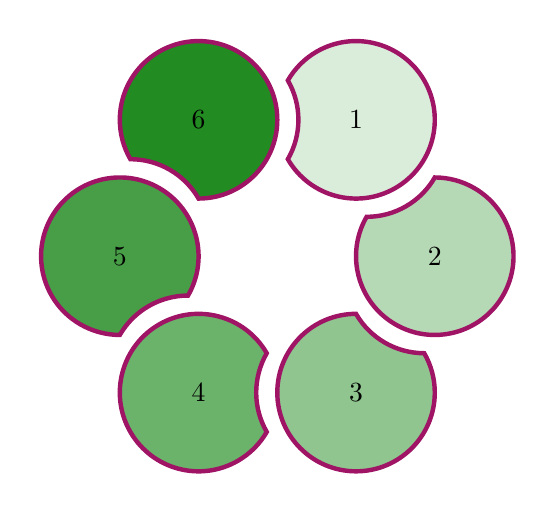
\begin{tikzpicture}
\wheelchart[
    data={},
    radius={2}{2},
    slices={(90:1) arc[start angle=-30,
        end angle=-90,radius=1]
        arc[start angle=-210,
        end angle=90,radius=1]--cycle;},
    slices style={
        /utils/exec={
            \pgfmathsetmacro
                {\WCcolornumber}
                {(\WCcount/
                    \WCtotalcount)*100}
        },
        ForestGreen!\WCcolornumber,
        draw=RedViolet,
        ultra thick
    },
    total count=6,
    value=1,
    wheel data=\WCcount
]{}
\end{tikzpicture}
\end{codeexample}
\begin{codeexample}[width=10cm]

\begin{tikzpicture}
\wheelchart[
    radius={2.7}{3.1},
    slices={(0,-0.3)--(0.3,0)--(0,0.3)
        --cycle;},
    value=1
]{\exampleforthismanual}
\wheelchart[
    data={},
    value=1
]{\exampleforthismanual}
\wheelchart[
    data={},
    radius={2}{2},
    slices={(0,0) circle[radius=0.4];},
    slices style=White,
    value=1
]{\exampleforthismanual}
\wheelchart[
    data={},
    radius={2}{2},
    slices={(0,0) circle[radius=0.3];},
    value=1,
    wheel data=\WCcount
]{\exampleforthismanual}
\end{tikzpicture}
\end{codeexample}
\end{key}
\begin{key}{/wheelchart/slices arc=\marg{value 1}\marg{value 2}}
This key sets both |slices end arc| and |slices start arc|. The effect of \meta{value 1} and \meta{value 2} is shown in the table below.

%\begin{codeexample}[width=10cm]
\def\exampleslicesarc#1#2{%
\begin{tikzpicture}[baseline={(0,0)}]
\draw[Red,ultra thick] (-1,0)--(1,0);
\pgfmathsetmacro{\angle}{atan(0.5*((1/(#1))-(#1)))}
\draw (-1,0)--({-(1-(#2))},0) arc[start angle={sign(#1)*180-\angle},end angle={\angle},radius={0.5*(1-(#2))*abs((1/(#1))+(#1))}]--(1,0);
\end{tikzpicture}%
}
\begin{tabular}{l|ccc}
 & $\text{\meta{value 2}}=-0.5$ & $\text{\meta{value 2}}=0$ & $\text{\meta{value 2}}=0.5$\\\hline
$\text{\meta{value 1}}=2$ & \exampleslicesarc{2}{-0.5} & \exampleslicesarc{2}{0} & \exampleslicesarc{2}{0.5}\\
$\text{\meta{value 1}}=1$ & \exampleslicesarc{1}{-0.5} & \exampleslicesarc{1}{0} & \exampleslicesarc{1}{0.5}\\
$\text{\meta{value 1}}=-1$ & \exampleslicesarc{-1}{-0.5} & \exampleslicesarc{-1}{0} & \exampleslicesarc{-1}{0.5}\\
$\text{\meta{value 1}}=-2$ & \exampleslicesarc{-2}{-0.5} & \exampleslicesarc{-2}{0} & \exampleslicesarc{-2}{0.5}\\
\end{tabular}
%\end{codeexample}
\begin{codeexample}[width=10cm]
\begin{tikzpicture}
\wheelchart[
    slices arc={1}{0}
]{\exampleforthismanual}
\end{tikzpicture}
\end{codeexample}
\begin{codeexample}[width=10cm]
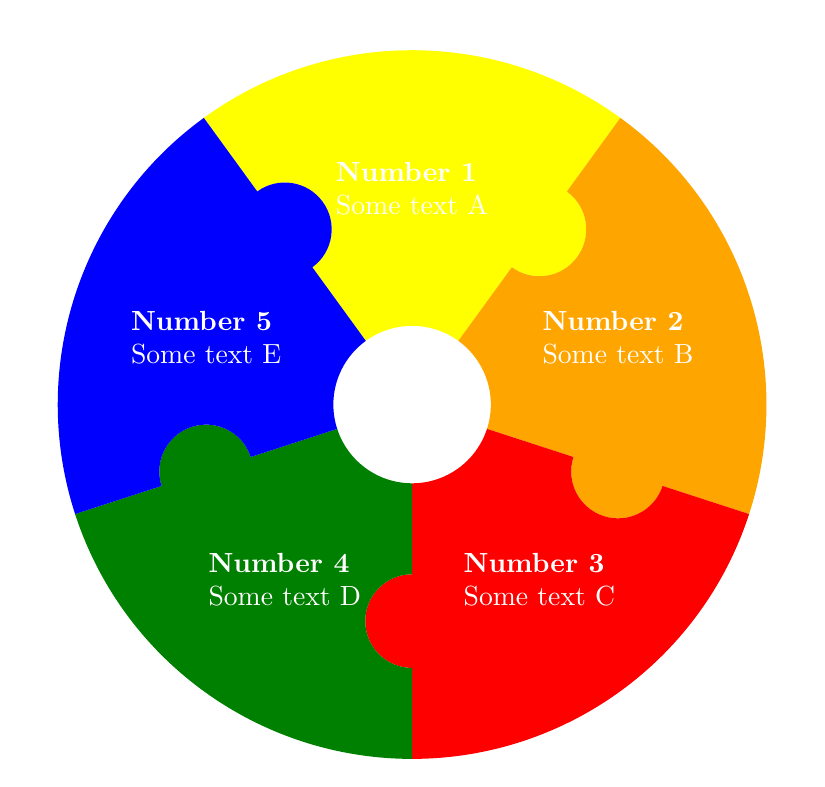
\begin{tikzpicture}
\wheelchart[
    data={},
    radius={1}{4.5},
    slices arc={1}{0.66},
    slices style=\WCvarA,
    start half,
    value=1,
    wheel data={%
        \textbf{Number \WCcount}\\%
        \WCvarB%
    },
    wheel data pos=0.5,
    wheel data style=White
]{%
    Yellow/{Some text A},
    Orange/{Some text B},
    Red/{Some text C},
    Green/{Some text D},
    Blue/{Some text E}%
}
\end{tikzpicture}
\end{codeexample}
\end{key}
\begin{key}{/wheelchart/slices arrow=\marg{value 1}\marg{value 2}}
This key is similar to the key |slices arc|.
\begin{codeexample}[width=10cm]
\begin{tikzpicture}
\wheelchart[
    gap=0.3,
    slices arrow={1}{-1}
]{\exampleforthismanual}
\end{tikzpicture}
\end{codeexample}
\end{key}
\begin{key}{/wheelchart/slices end arc=\marg{value 1}\marg{value 2}}
This key is similar to the key |slices arc| but only sets the end of the slice.
\end{key}
\begin{key}{/wheelchart/slices end arrow=\marg{value 1}\marg{value 2}}
This key is similar to the key |slices arrow| but only sets the end of the slice.
\begin{codeexample}[width=10cm]
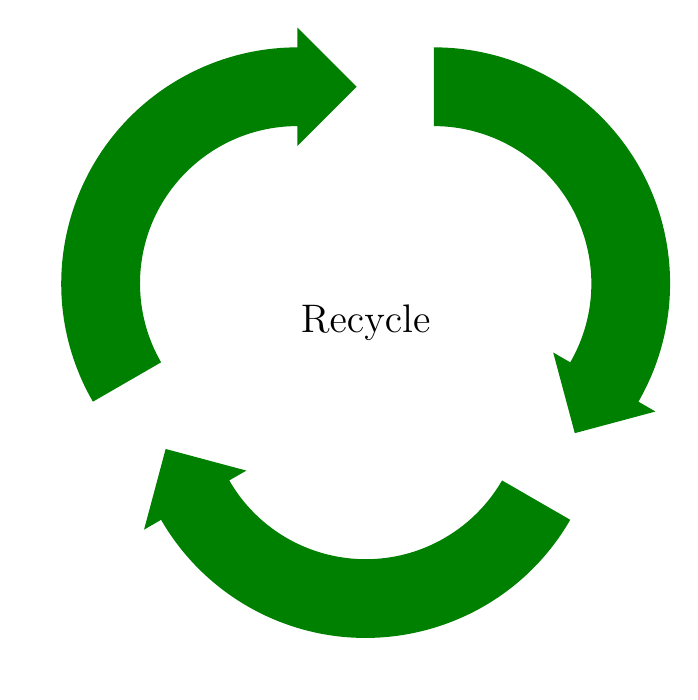
\begin{tikzpicture}
\wheelchart[
    data={},
    explode=1,
    middle={\Large Recycle},
    slices end arrow={1}{-0.5},
    slices style=Green,
    total count=3,
    value=1
]{}
\end{tikzpicture}
\end{codeexample}
\end{key}
\begin{key}{/wheelchart/slices start arc=\marg{value 1}\marg{value 2}}
This key is similar to the key |slices arc| but only sets the start of the slice.
\end{key}
\begin{key}{/wheelchart/slices start arrow=\marg{value 1}\marg{value 2}}
This key is similar to the key |slices arrow| but only sets the start of the slice.
\end{key}
\begin{stylekey}{/wheelchart/slices style=\marg{options} (initially \textbackslash WCvarB)}
This key defines the style of the slices of the wheelchart.
\end{stylekey}
\begin{key}{/wheelchart/start angle=\marg{angle} (initially 90)}
This key defines the \meta{angle} in degrees at which the first slice of the wheelchart starts.
\end{key}
\begin{key}{/wheelchart/start half=\marg{angle} (default 90)}
If this key is set then the middle of the first slice of the wheelchart is positioned at \meta{angle} in degrees.
\end{key}
\begin{key}{/wheelchart/title=\marg{text}}
This key contains the \meta{text} which will be placed above the wheelchart. The \meta{text} is placed in a node. The $x$ coordinate of this node is the $x$ coordinate of the center of the wheelchart, which is defined by the key |at|. In general, this is \emph{not} the same as the $x$ coordinate of the center of the |local bounding box| around the wheelchart. The $y$ coordinate of this node is |0.5| above the north of the |local bounding box| around the wheelchart. The style of this node is given as follows. First, the options |anchor=south,align=center| are given. Thereafter, the style of the key |title style| is added.
\end{key}
\begin{key}{/wheelchart/title left=\marg{text}}
This key contains the \meta{text} which will be placed above left of the wheelchart. The \meta{text} is placed in a node. This node is placed |0.5| above the north west of the |local bounding box| around the wheelchart. The style of this node is given as follows. First, the options |anchor=south west,align=left| are given. Thereafter, the style of the key |title left style| is added.
\end{key}
\begin{stylekey}{/wheelchart/title left style=\marg{options} (initially \normalfont empty)}
This key accepts a list of keys which will be applied to the node where the contents of the key |title left| is placed.
\end{stylekey}
\begin{stylekey}{/wheelchart/title style=\marg{options} (initially \normalfont empty)}
This key accepts a list of keys which will be applied to the node where the contents of the key |title| is placed.
\end{stylekey}
\begin{key}{/wheelchart/total angle=\marg{angle} (initially 360)}
This key defines the total \meta{angle} in degrees of the wheelchart.
\end{key}
\begin{key}{/wheelchart/total count=\marg{number}}
If this key is set then the number of slices of the wheelchart is determined by \meta{number}.
\begin{codeexample}[width=10cm,preamble={\usepackage{listofitems}}]
\readlist*\WCcolors{
    Rhodamine,RedOrange,OrangeRed
}
\setsepchar{ }
\readlist\WCdata{An example with the
    package \texttt{listofitems} where
    some keys are given using a list}
\begin{tikzpicture}
\wheelchart[
    data={\WCdata[\WCcount]},
    slices style={
        /utils/exec={
            \pgfmathsetmacro
                {\WCcolornumber}
                {int(Mod({\WCcount-1},
                    \WCcolorslen)+1)}
        },
        \WCcolors[\WCcolornumber]
    },
    total count={\WCdatalen},
    value=1
]{}
\end{tikzpicture}
\end{codeexample}
\begin{codeexample}[width=10cm,preamble={\usepackage{siunitx}}]
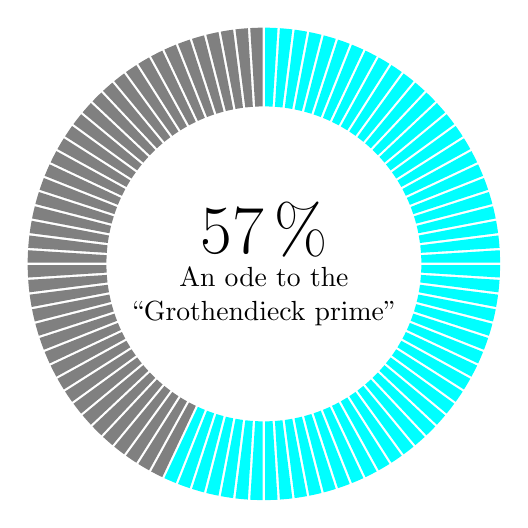
\begin{tikzpicture}
\def\n{57}
\wheelchart[
    data={},
    gap=0.015,
    middle={%
        {\Huge\qty{\n}{\percent}}\\%
        An ode to the\\%
        ``Grothendieck prime''%
    },
    slices style={
        /utils/exec={
            \ifnum\WCcount>\n
                \def\WCcolor{Gray}
            \else
                \def\WCcolor{Cyan}
            \fi
        },
        \WCcolor
    },
    total count=100,
    value=1
]{}
\end{tikzpicture}
\end{codeexample}
\end{key}
\begin{key}{/wheelchart/value=\marg{value} (initially \textbackslash WCvarA)}
This key defines the \meta{value} which corresponds to the size of each slice of the wheelchart.
\end{key}
\begin{key}{/wheelchart/wheel data=\marg{text}}
This key contains the \meta{text} which will be placed on top of each slice of the wheelchart. The \meta{text} is placed in a node. The style of this node is given as follows. First, the option |align=left| is given. Thereafter, the style of the key |wheel data style| is added.
\end{key}
\begin{key}{/wheelchart/wheel data pos=\marg{value} (initially 0.66)}
The radius of the polar coordinate at which the contents of the key |wheel data| is placed is given by the convex combination $\text{|wheel data pos|}\cdot\text{|outer radius|}+(1-\text{|wheel data pos|})\cdot\text{|inner radius|}$.
\end{key}
\begin{stylekey}{/wheelchart/wheel data style=\marg{options} (initially \normalfont empty)}
This key accepts a list of keys which will be applied to the node where the contents of the key |wheel data| is placed.
\end{stylekey}
\begin{stylekey}{/wheelchart/wheel lines=\marg{options} (initially \normalfont empty)}
If this key is set then lines with the style determined by this key will be drawn inside the slices of the wheelchart. The number of these lines depends on the value of the key |value|.

Below is the example from \cite[Subsection 7.6]{TtTaPGFp} recreated with the package |wheelchart|.
\begin{codeexample}[width=10cm]
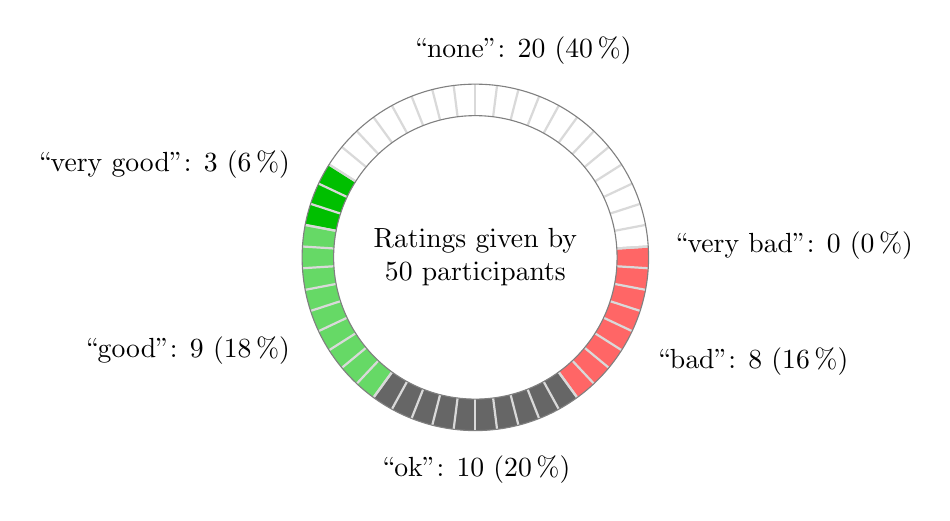
\begin{tikzpicture}
\colorlet{good}{green!75!black}
\colorlet{bad}{red}
\colorlet{neutral}{black!60}
\colorlet{none}{white}
\wheelchart[
    anchor xsep=15,
    contour=gray,
    data={``\WCvarC'': \WCvarA{} (\WCperc)},
    middle={Ratings given by\\\pgfmathprintnumber{\WCtotalnum}~participants},
    radius={1.8}{2.2},
    start half=270,
    wheel lines={black!15,thick}
]{%
    10/neutral/ok,
    9/good!60!white/good,
    3/good/{very good},
    20/none/none,
    0/bad/{very bad},
    8/bad!60!white/bad%
}
\end{tikzpicture}
\end{codeexample}
\end{stylekey}
\begin{thebibliography}{9}
\bibitem{JhcIparowcltopotPGFm}
Jake,
\emph{How can I produce a `ring (or wheel) chart' like that on page 88 of the {\upshape\pgfname} manual?},
\url{https://tex.stackexchange.com/questions/17898/how-can-i-produce-a-ring-or-wheel-chart-like-that-on-page-88-of-the-pgf-manu/18105#18105},
2011.
\bibitem{MpMP}
Jens-Uwe Morawski,
\emph{{\upshape\texttt{piechart}\textsf{MP}}},
Manual for Preliminary Version,
\url{https://ctan.org/pkg/piechartmp},
2002.
\bibitem{RSVpaaMfp}
Dominique Rodriguez, Michael Sharpe, Herbert Vo{\ss},
\emph{{\upshape\texttt{pstricks-add} \textsf{additionals Macros for} \texttt{pstricks}}},
Manual for version 3.92,
\url{https://ctan.org/pkg/pstricks-add},
2021.
\bibitem{Tumfdb}
Nicola L.C.~Talbot,
\emph{User Manual for datatool bundle version 2.32},
\url{https://ctan.org/pkg/datatool},
2019.
\bibitem{TtTaPGFp}
Till Tantau,
\emph{The \tikzname{} and {\upshape\pgfname} Packages},
Manual for version 3.1.9a,
\url{https://ctan.org/pkg/pgf},
2021.
\bibitem{XdPCbupp}
Yuan Xu,
\emph{Drawing Pie Chart by using {\upshape\texttt{pgf-pie}}},
Manual for version 0.6,
\url{https://ctan.org/pkg/pgf-pie},
2021.
\end{thebibliography}
\printindex
\end{document}